\chapter{Death, Life, And Love}

This chapter follows J. Krishnamurti's conversation with Dr. Alan W. Anderson on death, consciousness, reincarnation, immortality, and love. There are no blackboard frames or visual equations for this lecture, so the mathematical structure below is an editorial reconstruction of the spoken inquiry. We use compact notation only to keep the distinctions clear: the source of the chapter remains the dialogue itself.

\section{The Fear Around Death}

Anderson begins by returning to the previous conversation. They had been speaking of consciousness and death in relation to living as a total movement, and reincarnation had just been touched when the earlier dialogue ended. Krishnamurti does not begin by defining death. He begins with fear.

The word death is not ordinarily part of daily conversation. It is avoided, postponed, softened, even hidden cosmetically. The point is not merely social. If the mind is frightened of death, then the inquiry is already distorted. It will look for consolation, continuity, belief, or escape before it has seen the fact.

So the first condition of the chapter is:

\begin{equation}
\text{understanding death}
\quad\text{requires}\quad
\text{freedom from fear}.
\end{equation}

This is the first reversal. Death is usually treated as the negation of life. Krishnamurti speaks instead of the beauty, strength, and vitality of death. That phrase should not be converted into a doctrine. It is a signpost: if death is approached without fear, it may not be merely an end outside life, but a movement within living itself.

\section{Belief, Preparation, And The Question Of Fact}

Before asking what death is, the dialogue clears away inherited answers. Krishnamurti names three large historical forms. The ancient Egyptians prepared for death by carrying forward the goods of life. Reincarnation, as commonly believed, imagines continuation in another birth. Resurrection imagines another mode of survival after the grave.

These answers differ culturally, but in the lecture they share one structure. They extend the known.

\begin{align}
\text{preparation for death} &\Rightarrow \text{carry the known forward}, \\
\text{reincarnation as belief} &\Rightarrow \text{continue the known later}, \\
\text{resurrection as belief} &\Rightarrow \text{preserve the known beyond the grave}.
\end{align}

Krishnamurti then asks for the fact. Apart from the organism, what dies? The body may last eighty, ninety, or a hundred years if cared for, but the question remains: for what kind of life? A life of quarrel, bitterness, jealousy, futility, and fear would merely extend confusion.

At this point Anderson supplies a link to the previous inquiry: all this is the content of consciousness. The lecture then becomes more exact. The fear of death is not primarily fear of an unknown abstraction. It is fear of losing what one knows.

\begin{equation}
\text{fear of death}
\sim
\text{fear of losing the known}.
\end{equation}

The known includes wife, house, property, status, belief, acquired knowledge, memory, and the whole structure called ``my life.'' The inquiry into death has therefore become an inquiry into consciousness.

\section{The Content Of Consciousness As The Known}

Let us introduce a compact notation. It is not a formula from a blackboard; it is a way of preserving the spoken structure.

\begin{definition}
Let \(C\) denote the content of consciousness: attachment, dependency, acquisition, power, position, anxiety, fear, pleasure, knowledge, memory, inherited influence, and the hidden as well as the conscious material of the mind.
\end{definition}

The dialogue repeatedly identifies this content with the known and with the me. In shorthand,

\begin{equation}
C \equiv \text{the known} \equiv \text{the me}.
\end{equation}

This is the central relation of the chapter. It must be read carefully. Krishnamurti is not constructing a psychological theory in technical language. He is pointing out that what we call the self is not separate from the accumulated content of consciousness. The me is not standing outside the content and looking at it. The me is that content.

This changes the question of death. Death is not only the event that happens to the organism. Psychologically, death becomes the ending of the content that gives consciousness its frontier.

\begin{equation}
\text{emptying } C
\Rightarrow
\text{ending the limitation made by } C.
\end{equation}

Krishnamurti is careful about this. Emptying the content is not a brutal cutting off. It is not a violent act of detachment. He uses attachment as an example: if I am attached to property, a person, a book I have written, or knowledge I have acquired, then the struggle to become detached only begins another battle. The battle itself becomes part of consciousness.

\subsection{Question \& Answer}

\paragraph{Question.}
Can the content of consciousness be totally emptied?

\paragraph{Answer.}
Only if we first see what the content is and how it acts. The emptying is not suppression, not forced detachment, and not the cultivation of an opposite state. Attachment breeds pain; the desire to become detached breeds conflict; that conflict is again content. So the question becomes sharper: can the whole content be observed, including its hidden and unconscious layers, without turning that observation into another struggle?

The working relation is:

\begin{align}
\text{attachment} &\Rightarrow \text{pain}, \\
\text{will to detach} &\Rightarrow \text{conflict}, \\
\text{conflict} &\subset C.
\end{align}

Therefore the content cannot be emptied by adding another movement of the same content. This is why the dialogue next turns to analysis.

\section{Why Analysis Cannot Empty The Mind}

Krishnamurti now enlarges the field. There is conscious content: house, property, wife, children, job, things acquired, things learned. There is also deeper content: racial, collective, acquired, unconscious, gathered through pressure, influence, and the strains of living in a corrupt world. Anderson calls this both personal and impersonal.

The natural modern answer is analysis. We suppose that if each layer is analyzed, the content will be exposed and perhaps dissolved. Krishnamurti rejects this answer with the phrase ``analysis, paralysis.'' The point is not rhetorical. It has a structure.

\begin{proposition}
Analysis cannot empty the content of consciousness because analysis depends on division, time, and memory.
\end{proposition}

\begin{proof}
The argument in the dialogue may be written as a sequence.

\begin{enumerate}
\item Analysis begins by positing an analyser and the analysed.
\item The analyser is not outside consciousness; the analyser is a fragment of the same content.
\item Thus the analyser is the analysed:
\begin{equation}
\text{analyser} = \text{analysed}.
\end{equation}
\item Analysis requires duration. It takes time to unearth, uncover, interpret, and continue.
\item Every analysis is incomplete, or at least uncertain of completion.
\item The incomplete result is carried forward as memory.
\item That memory then analyzes the next incident.
\item Therefore analysis reproduces the continuity it claims to end.
\end{enumerate}

In compact form:
\begin{equation}
\text{analysis}
\Rightarrow
\text{division}
\Rightarrow
\text{time}
\Rightarrow
\text{incompletion}
\Rightarrow
\text{memory}
\Rightarrow
\text{further analysis}.
\end{equation}

This is why analysis becomes paralysis. It is a movement within \(C\), not an ending of \(C\).
\end{proof}

The force of the argument is that analysis can never be a complete act. If the mind sees that, analysis falls away. But then the lecture reaches its next real question.

\subsection{Question \& Answer}

\paragraph{Question.}
If analysis falls away, what is the mind to do with the content?

\paragraph{Answer.}
It has to be emptied; otherwise there is mere continuity. But it cannot be emptied by the analyser, because the analyser is part of the analysed. The mind must see the content totally, not fragment by fragment. This is why Krishnamurti asks, ``How is that to be done?'' The question opens the next construction: the map of consciousness.

\begin{figure}
\centering
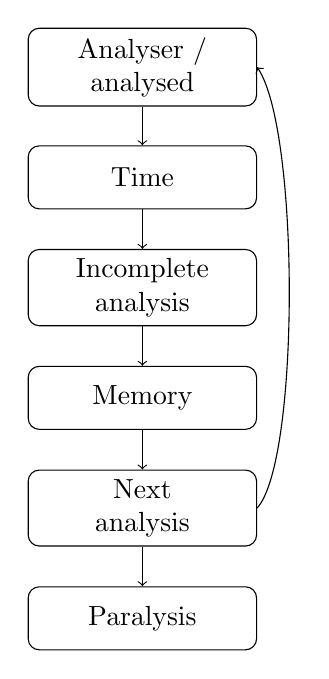
\begin{tikzpicture}[scale=1.0]
\node[draw, rounded corners, align=center, minimum width=2.9cm, minimum height=0.8cm] (a) at (0,0) {Analyser /\\ analysed};
\node[draw, rounded corners, align=center, minimum width=2.9cm, minimum height=0.8cm] (t) at (0,-1.4) {Time};
\node[draw, rounded corners, align=center, minimum width=2.9cm, minimum height=0.8cm] (i) at (0,-2.8) {Incomplete\\ analysis};
\node[draw, rounded corners, align=center, minimum width=2.9cm, minimum height=0.8cm] (m) at (0,-4.2) {Memory};
\node[draw, rounded corners, align=center, minimum width=2.9cm, minimum height=0.8cm] (n) at (0,-5.6) {Next\\ analysis};
\node[draw, rounded corners, align=center, minimum width=2.9cm, minimum height=0.8cm] (p) at (0,-7.0) {Paralysis};

\draw[->] (a) -- (t);
\draw[->] (t) -- (i);
\draw[->] (i) -- (m);
\draw[->] (m) -- (n);
\draw[->] (n) -- (p);
\draw[->] (n.east) .. controls (2.0,-5.0) and (2.0,-0.8) .. (a.east);
\end{tikzpicture}
\caption{The analysis loop reconstructed from the dialogue: division, time, incompletion, memory, repeated analysis, and paralysis.}
\end{figure}

\section{The Whole Map Without Direction}

The alternative is not another technique. Krishnamurti gives an image: reading a map. If we want to go in a direction, we look only for a route. We do not see the whole map. But if there is no direction, we can simply look.

This matters because direction is already choice. Choice selects, excludes, measures, and pursues. The mind then sees only the part relevant to its aim. But the question here is whether the whole content can be exposed.

Let \(W\) denote the whole map of consciousness. Let \(D\) denote directed search. Let \(A_c\) denote choiceless awareness. Then the contrast is:

\begin{align}
D(W) &\Rightarrow \text{a route through the map}, \\
A_c(W) &\Rightarrow \text{the whole map exposed}.
\end{align}

This notation should not be overread. It simply preserves the distinction. Directed attention narrows; choiceless awareness does not choose a path. Krishnamurti says that such awareness gives tremendous energy to go beyond the content.

\begin{equation}
A_c(C)
\Rightarrow
\text{energy to go beyond } C.
\end{equation}

That is the hinge of the chapter. Analysis attempts to solve the content through time. Choiceless awareness sees the content without time as a method.

\begin{figure}
\centering
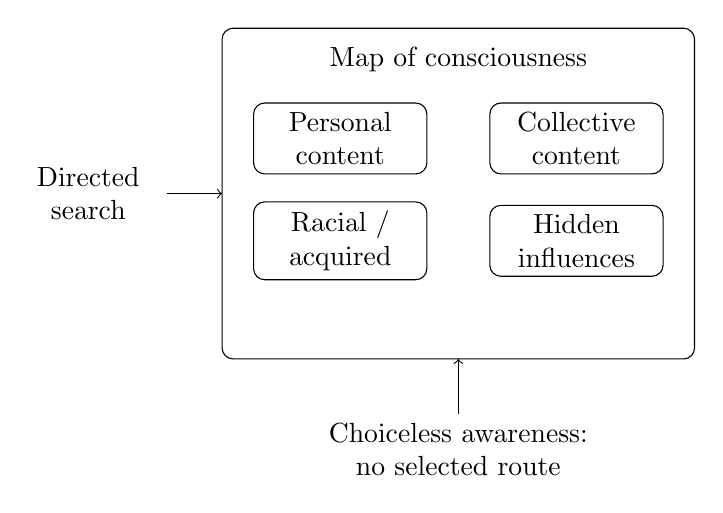
\begin{tikzpicture}[scale=1.0]
\draw[rounded corners] (-3.0,0.0) rectangle (3.0,4.2);
\node[align=center] at (0,3.8) {Map of consciousness};

\node[draw, rounded corners, align=center, minimum width=2.2cm] at (-1.5,2.8) {Personal\\ content};
\node[draw, rounded corners, align=center, minimum width=2.2cm] at (1.5,2.8) {Collective\\ content};
\node[draw, rounded corners, align=center, minimum width=2.2cm] at (-1.5,1.5) {Racial /\\ acquired};
\node[draw, rounded corners, align=center, minimum width=2.2cm] at (1.5,1.5) {Hidden\\ influences};

\draw[->] (-3.7,2.1) -- (-3.0,2.1);
\node[align=center] at (-4.7,2.1) {Directed\\ search};

\draw[->] (0,-0.7) -- (0,0.0);
\node[align=center] at (0,-1.15) {Choiceless awareness:\\ no selected route};

\end{tikzpicture}
\caption{The map metaphor: directed search sees a route; choiceless awareness looks at the whole field of content.}
\end{figure}

\section{Reincarnation Now, Or Continuity As A Stream}

The conversation now returns to reincarnation, but not as it appeared at the beginning. At first it was one of several beliefs about survival. Now the question has been transformed by the inquiry into content.

Krishnamurti's reversal is simple: people speak of reincarnating in a next life, but not of incarnating now. To incarnate now would mean to die to the content now. To be reborn or regenerated is not postponed to a future life; it is tied to the ending of \(C\).

\begin{equation}
\text{incarnation now}
\Leftrightarrow
\text{dying to } C \text{ now}.
\end{equation}

If the content is not emptied, it continues. Krishnamurti gives the image of a river: the content of me is not very different from the content of you. It is slightly modified by conditioning and environment, but essentially it is the same human consciousness. Unless it is emptied, it goes on like a stream, collecting and accumulating struggle, pain, unhappiness, fear, and confusion.

\begin{equation}
C_{\text{unemptied}}
\Rightarrow
\text{continuity as stream}.
\end{equation}

The stream image must be handled carefully. The lecture does not ask us to build a metaphysical system. It asks us to see continuity. Mediums and seances are mentioned as expressions arising from that continuing stream of content. But the person who has observed and emptied consciousness does not belong to that stream.

\begin{equation}
C_{\text{emptied}}
\Rightarrow
\text{not belonging to the stream}.
\end{equation}

Then living becomes new each moment because there is no accumulation of the me that must be expressed. Krishnamurti phrases it as living every minute and dying every minute.

\begin{figure}
\centering
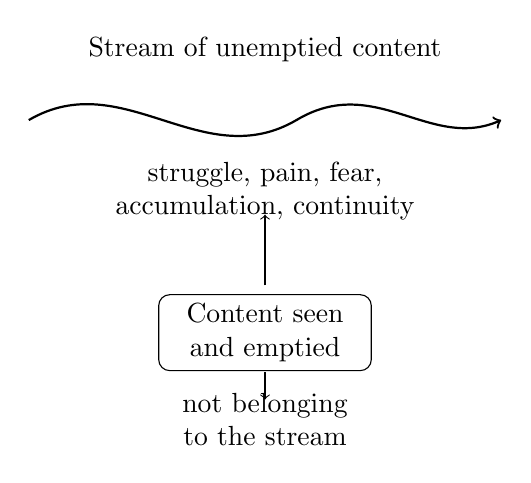
\begin{tikzpicture}[scale=1.0]
\draw[thick, ->] (-3.0,0) .. controls (-1.8,0.7) and (-0.8,-0.7) .. (0.4,0)
                     .. controls (1.4,0.6) and (2.1,-0.4) .. (3.0,0);
\node[align=center] at (0,0.9) {Stream of unemptied content};
\node[align=center] at (0,-0.9) {struggle, pain, fear,\\ accumulation, continuity};

\node[draw, rounded corners, align=center, minimum width=2.7cm] at (0,-2.7) {Content seen\\ and emptied};
\draw[->] (0,-2.1) -- (0,-1.2);

\node[align=center] at (0,-3.8) {not belonging\\ to the stream};
\draw[->] (0,-3.2) -- (0,-3.55);
\end{tikzpicture}
\caption{The stream of continuing content and the different movement of a mind that has emptied that content.}
\end{figure}

\section{Immortality, Beauty, And The Field Of Time}

The dialogue next asks: what is immortality? Krishnamurti approaches the question by negation. Immortality is not in the book, the painting, the cathedral, the statue, the family name, the righteous life, the doctrine, the savior invented by thought, or the gods made in man's image. All these are vulnerable to destruction. They are corruptible because they are made within time.

The compact relation is:

\begin{equation}
\text{time} = \text{thought}.
\end{equation}

Again, this is not a physical statement about clocks. It is a psychological statement within this inquiry. Thought creates images, symbols, ideals, buildings, names, and objects through which the self tries to continue.

\begin{equation}
\text{what thought creates}
\subset
\text{the field of time}.
\end{equation}

And therefore:

\begin{equation}
\text{thought-made immortality}
\subset
\text{the field of time}.
\end{equation}

What belongs to time can be destroyed. Earthquake, fire, accident, decay, and violence can undo it. Even if an object lasts, the self that tries to immortalize itself through the object remains bound to thought.

\subsection{Question \& Answer}

\paragraph{Question.}
If immortality is not in works, buildings, beliefs, names, or thought-made gods, what is it?

\paragraph{Answer.}
Krishnamurti distinguishes the object of beauty from beauty itself. A cathedral, poem, sculpture, or painting may perish. The object can be destroyed. But beauty itself is not the object. Beauty itself is not grasped by the mind as content, and Krishnamurti says it is not in the field of consciousness.

\begin{equation}
\text{beautiful object} \in \text{field of time},
\qquad
\text{beauty itself} \notin \text{field of consciousness}.
\end{equation}

Anderson notices the reversal. We usually think beauty dies when the thing we cherish dies. The dialogue turns that upside down: perhaps beauty has let that expression go. The object perishes; beauty is not imprisoned in the object.

\begin{table}
\centering
\begin{tabular}{|p{0.43\linewidth}|p{0.43\linewidth}|}
\hline
Within the field of time & Not treated as within time \\
\hline
Books, paintings, statues, cathedrals & Beauty itself \\
\hline
Family name, reputation, works & The ending of the me \\
\hline
Gods and ideals made by thought & A state not made by thought \\
\hline
Continuity of accumulated content & Living without psychological accumulation \\
\hline
\end{tabular}
\caption{A compact reconstruction of the lecture's contrast between thought-made immortality and what is not contained by thought.}
\end{table}

\section{Living, Love, Death, And Education}

The final movement gathers the whole dialogue. Death is not merely the future event that happens to the organism. The present, in this inquiry, is the death of the content. That means no psychological tomorrow as the continuation of accumulation. This sounds absurd if the mind assumes analysis, progress, and time as the only means of change. But it is exactly the point.

The relations are:

\begin{align}
\text{living} &= \text{dying}, \\
\text{dying to time} &= \text{love}, \\
\text{living},\ \text{love},\ \text{death}
&\Rightarrow
\text{one indivisible movement}.
\end{align}

The transcript likely misrenders one phrase as ``dying to the mean.'' In context, the sense is dying to the me. Love is not what thought says love is: not possession, not pleasure, not merely sex, not the image of another. Love is linked here with dying to time, dying to the me, and therefore dying to the content that divides.

This brings the lecture to education. If from childhood we are taught only the cultivation of thought, then knowledge becomes the field of psychological safety. To die to all that then appears insane, because knowledge has become part of me. The question becomes whether children and students can be educated to live differently: not without practical knowledge, but without making knowledge the refuge of the self.

The movement can be summarized as a final chain:

\begin{equation}
\text{thought as security}
\Rightarrow
\text{fear of not knowing}
\Rightarrow
\text{clinging to } C
\Rightarrow
\text{continuity of the me}.
\end{equation}

Against that stands the other movement:

\begin{equation}
\text{actual perception of what is}
\Rightarrow
\text{ending of dissipation}
\Rightarrow
\text{energy in action}
\Rightarrow
\text{transformation not in time}.
\end{equation}

The late transcript contains garbled speaker labels and a brief foreign-language fragment, but the surrounding point is clear enough: transformation is not within the field of time and knowledge. It is not produced by an outside agency. It is the same energy no longer dissipated.

\section{Summary}

The dialogue begins with death and ends with education, but its real spine is the movement of consciousness as content. Fear of death is fear of losing the known. The known is the content of consciousness, and that content is the me. Analysis cannot empty the content because the analyser is the analysed and analysis works through time, memory, and incompletion.

The alternative is not another method. It is the seeing of the whole map without direction or choice. From there reincarnation is reworked as incarnation now: if the content is not emptied it continues like a river; if it is emptied there is no belonging to that stream. Immortality is then separated from thought-made objects and placed with beauty itself, not the object of beauty. The conclusion is stark: living, love, and death are not separate movements in time, but one indivisible movement when the content of the me comes to an end.